\section{The local metric and a compact comparison family}
\label{sec:comparison-metrics}

The local singularity fixes a useful smooth metric in its original
holomorphic presentation. We first calculate that metric, including
the normalization of its curvature charge, and then construct a
family on the compact bundle. Its parameter is independent of flow
time at this stage.

\subsection{An explicit metric at a reduced point}

On $\CC^2$ use the Euclidean conventions of
Section~\ref{sec:geometry}, the inclusion $z=(z_1,z_2)^{\mathsf t}$
and the quotient $(-z_2,z_1)$. A constant unitary sign change gives
the presentation in \eqref{eq:normal-reference}. For $a>0$ and
$s=|z|^2$, put
\begin{equation}\label{eq:local-metric}
 \begin{aligned}
 w_a&=\frac{a}{s+a},\qquad P=\frac{zz^*}{s},\\
 H_a^{\mathrm{loc}}
     &=w_aP+w_a^{-1}(I-P)
       =\frac{s+a}{a}I-\frac{s+2a}{a(s+a)}zz^* .
 \end{aligned}
\end{equation}
The final expression is defined also at the origin.

\begin{lemma}\label{lem:local-metric}
The metric \eqref{eq:local-metric} is smooth and positive on
$\CC^2$, equals $I$ at zero, and has determinant one. Its Chern
connection satisfies $i\Lambda_{\omega_E}F_a=0$ and is anti-self-dual
for the complex orientation. With the stated real tensor norms,
\begin{equation}\label{eq:local-densities}
 \begin{aligned}
 u_a^{\mathrm{loc}}&=\frac{as}{s+a},&
 |D'_az|^2&=\frac{4a^3}{(s+a)^3},&
 |F_a|^2&=\frac{48a^2}{(s+a)^4}.
 \end{aligned}
\end{equation}
In particular the total curvature energy is $8\pi^2$. For a
Euclidean radius-$R$ ball,
\begin{align}
 \int_{B_R}|D'_az|^2\,\dd V_E
   &=2\pi^2a^2\frac{R^4}{(R^2+a)^2},
       \label{eq:local-section-energy}\\
 \int_{B_R}u_a^{\mathrm{loc}}\,\dd V_E
   &=\pi^2a\left\{\frac{R^4}{2}-aR^2
                         +a^2\log(1+R^2/a)\right\},
       \label{eq:local-mass}\\
 \int_{B_R}|F_a|^2\,\dd V_E
   &=8\pi^2\mathfrak F(R/\sqrt a),\qquad
 \mathfrak F(t)=\frac{t^4(t^2+3)}{(1+t^2)^3}.
       \label{eq:local-curvature-energy}
\end{align}
\end{lemma}

\begin{proof}
The two projections in \eqref{eq:local-metric} have reciprocal
positive eigenvalues. Its smooth matrix expression extends
positivity and determinant one across zero.
Use the holomorphic-frame convention
$D'=\partial+H^{-1}\partial H$ and
$F=\db(H^{-1}\partial H)$.
The metric is equivariant under simultaneous unitary changes of
base and fibre, so it suffices to calculate at $z=(r,0)$.

For a general radial $w>0$, set $f=\log w$ and
$F_{\bar j k}=\partial_{\bar z_j}(H^{-1}\partial_{z_k}H)$.
Differentiating the projection expression gives
\[
 F_{\bar1 1}=(f'+sf'')\diag(1,-1),\qquad
 F_{\bar2 2}=\left(f'+\frac{1-w^2}{s}\right)\diag(1,-1).
\]
For example, $H^{-1}\partial_{z_2}H$ has lower-left entry
$(w^2-1)/r$ at the axis. When taking the next derivative,
the derivative of $H^{-1}$ contributes
$-(w-w^{-1})^2/s$ to the first diagonal entry. Including
this term gives the displayed second formula. The contraction
therefore vanishes exactly when
\[
                  s^2f''+2sf'+1-e^{2f}=0.
\]
For $f=\log a-\log(s+a)$, the numerator after multiplication
by $(s+a)^2$ is
$s^2-2s(s+a)+(s+a)^2-a^2=0$.
The curvature is trace-free and of type $(1,1)$, so its
primitivity is equivalent to anti-self-duality.

The inclusion lies in the range of $P$, which gives its norm.
At the axis its covariant derivative has coefficient columns
$(w_a,0)^{\mathsf t}$ and $(0,w_a^2)^{\mathsf t}$.
Each has squared $H_a^{\mathrm{loc}}$-norm $w_a^3$.
Since $|\dd z_j|^2=2$, the section-energy density is $4w_a^3$.
For a radial scalar function $U(s)$,
$-\Delta_0U=4sU''+8U'$. Substitution also verifies
$-\Delta_0u_a^{\mathrm{loc}}=2|D'_az|^2$.

For completeness, put $c=a/(s+a)^2$. The four curvature
coefficients in the holomorphic frame at the axis are
\[
 \begin{array}{ll}
 F_{\bar1 1}=-c\diag(1,-1),&
 F_{\bar2 2}= c\diag(1,-1),\\[2pt]
 F_{\bar1 2}=-\dfrac{2a^2}{(s+a)^3}E_{21},&
 F_{\bar2 1}=-\dfrac{2}{s+a}E_{12}.
 \end{array}
\]
Conjugating by $H_a^{1/2}$ to a unitary frame makes the
two off-diagonal coefficients both $-2c$. The four
forms $\dd\bar z_j\wedge\dd z_k$ are mutually orthogonal
and have squared norm four. The sum of the squared matrix
norms is $12c^2$, giving $|F_a|^2=48c^2$.

The radial Euclidean measure is $\pi^2s\,\dd s$.
Integrating the three densities gives
\eqref{eq:local-section-energy}--\eqref{eq:local-curvature-energy}.
In particular
\[
 \int_{\CC^2}|F_a|^2\,\dd V_E
       =48\pi^2\int_0^\infty\frac{t}{(1+t)^4}\,\dd t
       =8\pi^2 .
\]
With our skew-Hermitian trace convention, anti-self-duality
gives $\tr(F_a\wedge F_a)=|F_a|^2\dd V_E$, fixing the
positive charge sign.
\end{proof}

\begin{figure}[htbp]
\centering
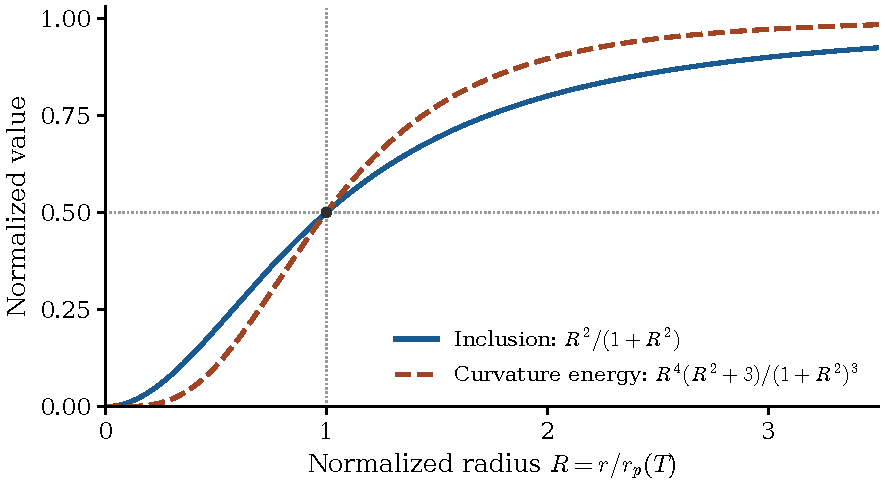
\includegraphics[width=.94\textwidth]{figures/local_profiles.pdf}
\caption{The exact local inclusion profile and the fraction of the
charge-one curvature energy inside a ball. Each takes the value
\(1/2\) at normalized radius one. The curves depict the explicit
local metric; their identification as actual-flow limits is proved
in Sections~\ref{sec:actual-comparison} and \ref{sec:energy-curvature}.}
\label{fig:local-profiles}
\end{figure}

The normalized inclusion is $s/(s+a)$. Its half-height radius
is $\sqrt a$, and \eqref{eq:local-curvature-energy} has half
its total energy at the same radius because $\mathfrak F(1)=1/2$.
Under $z=\sqrt a\,y$ the curvature measure becomes exactly
$48(1+|y|^2)^{-4}\dd V_y$. These are identities for a stationary
local metric. A nonconstant choice $a=a(T)$ gives a nonzero
metric velocity while the curvature contraction remains zero,
so time dependence requires a separate compact correction.

\subsection{A family on the original compact bundle}

Return to the general extension \eqref{eq:extension} and fix
any smooth $H_0$ with determinant $h_{\det}$. Using $h_L$
for the adjoint of the inclusion, put
$S=\iota\iota^\dagger$ and $u_0=\tr S=\iota^*H_0/h_L$.
Then $S^2=u_0S$, and both $S$ and $u_0$ vanish on $\Sigma$.
Define
\begin{equation}\label{eq:compact-metric}
 T_a=\frac{u_0+a}{a}I-\frac{u_0+2a}{a(u_0+a)}S,
                 \qquad H_a=H_0T_a,\qquad a>0 .
\end{equation}
This formula is intrinsic on $V$. The product $H_0T_a$
means the Hermitian form with that matrix in a local frame.

\begin{proposition}\label{prop:compact-family}
The metrics \eqref{eq:compact-metric} are smooth, positive
and have determinant $h_{\det}$. If
$e_a=|D'_{H_a\otimes h_L^{-1}}\iota|^2$, then
\begin{equation}\label{eq:compact-identities}
 u_a=\frac{au_0}{u_0+a},\qquad
 e_a=\left(\frac{a}{u_0+a}\right)^3e_0,\qquad
 Z_a=av_0-a^2\int_X\frac{\dd V}{u_0+a}.
\end{equation}
For every finite $W$, $Z_a/a\to v_0$ and $u_a/Z_a\to1/v_0$
smoothly on compact subsets of $U$.
If $W$ is reduced, then
\begin{equation}\label{eq:static-leading}
 \mathcal E_a=C(H_0)a^2+o(a^2),\qquad
 C(H_0)=\pi^2\sum_{p\in\Sigma}\frac{\tr Q_p}{\det Q_p},
 \qquad
 Z_a=av_0-a^2 I_0+o(a^2),
\end{equation}
where $I_0=\int_Xu_0^{-1}\dd V<\infty$.
Furthermore $C(H_0)\ge2\pi^2\sigma$, with equality for the
reference metric of Lemma~\ref{lem:normalized-reference}.
\end{proposition}

\begin{proof}
On $U$, $P=S/u_0$ is the $H_0$-orthogonal projection onto
the inclusion line, and
\[
 T_a=\frac{a}{u_0+a}P+\frac{u_0+a}{a}(I-P).
\]
Its eigenvalues are positive reciprocals. The global expression
\eqref{eq:compact-metric} is smooth at $\Sigma$, where $T_a=I$.
This proves the metric and determinant assertions. Evaluation
on the inclusion gives the first formula in
\eqref{eq:compact-identities}, and integration gives the last.

To calculate the full derivative, let $\tau$ be the
$H_0$-orthogonal right inverse of $q$ on $U$ and write
$\db\tau=\iota\beta$. The same splitting is orthogonal for
$H_a$; its line and quotient metrics are
$(u_ah_L,u_a^{-1}h_M)$. For any metric diagonal in this
splitting with induced inclusion norm $u$, the tangential and
normal Chern derivatives are orthogonal, and their squared
norms are respectively
\begin{equation}\label{eq:full-inclusion-energy}
             e=\frac{|\partial u|^2}{u}+u^3|\beta|_0^2 .
\end{equation}
Here $|\beta|_0$ uses the fixed metric $h_Lh_M^{-1}$ and
the base metric. Indeed the tangential component is
$(\partial\log u)\iota$, while the adjoint of the off-diagonal
Dolbeault block has the two quotient weights and the additional
inclusion weight. Since
$\partial u_a=a^2\partial u_0/(u_0+a)^2$, both terms in
\eqref{eq:full-inclusion-energy} acquire the factor
$a^3/(u_0+a)^3$. This proves the middle identity on $U$,
and smoothness extends it across $\Sigma$.

The bound $0\le u_a/a\le1$ and dominated convergence give
$Z_a/a\to v_0$. On each compact subset of $U$, the rational
formula converges with every fixed derivative.

At a reduced zero, $e_0(p)=2\tr Q_p$ because the
connection terms multiply the vanishing inclusion and
$|\dd z_j|^2=2$. On a small ball $u_0\asymp|z|^2$ and
$e_0$ is bounded. Substitute $z=\sqrt a\,y$ in the
energy identity and divide its integral by $a^2$.
The integrand, extended by zero outside the rescaled ball,
is bounded by $C(1+c|y|^2)^{-3}$, integrable on $\RR^4$.
It converges to $e_0(p)(1+y^*Q_py)^{-3}$. Thus its
integral tends to
\[
 \frac{e_0(p)}{\det Q_p}
       \int_{\CC^2}(1+|y|^2)^{-3}\,\dd V_y
                  =\pi^2\frac{\tr Q_p}{\det Q_p}.
\]
On the fixed exterior the energy is $O(a^3)$.
Summing proves the energy assertion. Also $u_0^{-1}$ is
locally bounded by $C|z|^{-2}$, which is integrable in
four real dimensions. Dominated convergence in the last
formula of \eqref{eq:compact-identities} gives the mass
expansion.

Finally $\det Q_p=d_p$ is fixed, and
$\tr Q_p\ge2\sqrt{d_p}$, with equality exactly when
$Q_p=\sqrt{d_p}\,I$. The normalized reference metric has
this value at every point, proving the last assertion.
\end{proof}

\subsection{Matching the local and exterior descriptions}

From now on, when $W$ is reduced we use the one normalized
reference metric in Lemma~\ref{lem:normalized-reference}.
On its local ball, put $s=|z|^2$, $c=c_p(z)$ and
$h=\sqrt{h_Lh_M}$. The compact metric is
\begin{equation}\label{eq:compact-local-expression}
 H_a=h\{wP+w^{-1}(I-P)\},\qquad
 w=\frac{a}{a+cs},\qquad
 u_a=\frac{acs}{a+cs},
\end{equation}
where $P$ projects onto $(z_1,-z_2)^{\mathsf t}$.
At the scale $z=\sqrt{a/\lambda_p}\,y$, its smooth matrix
expression converges in every fixed number of derivatives
on compact $y$-sets to
\begin{equation}\label{eq:unit-local-profile}
 H_{\mathrm{loc}}(y)
   =(1+|y|^2)I-\frac{|y|^2+2}{1+|y|^2}YY^*,
                 \qquad Y=(y_1,-y_2)^{\mathsf t}.
\end{equation}
Indeed $u_0/a\to|y|^2$, $H_0\to I$, and
$S/a\to YY^*$ smoothly there; all denominators are bounded
below. The rescaled base metric tends to the Euclidean
metric. This is the local metric of
Lemma~\ref{lem:local-metric} at parameter one, with its
fixed unitary sign change.

On the compact exterior $u_a/a\to1$. The exact common
formula \eqref{eq:compact-metric} joins these descriptions
without changing the holomorphic bundle or its inclusion.
In particular
\begin{equation}\label{eq:balanced-static}
             Z_a=av_0+O(a^2),\qquad
             \mathcal E_a=2\pi^2\sigma a^2+o(a^2).
\end{equation}
These are static identities and asymptotics. The next
sections estimate the mean curvature, correct its
orthogonal component and prove the parameter control
needed to compare the resulting path with actual flow.
